
\documentclass{mcmthesis}
\mcmsetup{
  CTeX = false,
  tcn = 0000000,
  problem = A,
  sheet = true,
  titleinsheet = true,
  keywordsinsheet = true,
  titlepage = false,
  abstract = true
}
\usepackage{indentfirst}
\setlength{\parindent}{2em}
\renewcommand{\rmdefault}{cmr}
\renewcommand{\sfdefault}{cmss}
\usepackage{amsmath,amssymb,booktabs,tabularx,longtable,float,graphicx,array}
\usepackage{enumitem}
\usepackage{hyperref}
\usepackage{lastpage}
\usepackage{caption}
\usepackage{placeins}
\setlength{\headheight}{15pt}
\setlength{\parskip}{2pt}
\setlist[itemize]{leftmargin=1.7em,itemsep=2pt,topsep=3pt}
\graphicspath{{../figures/}}
\title{Clearing Every Room: Optimal Responder Sweep Routing for Emergency Evacuation}

\begin{document}
\begin{abstract}
When a fire or gas leak forces a building evacuation, trained responders must sweep every room to confirm that no one is left behind, and the clock is measured in seconds. We build an evidence-traceable sweep-routing model for multi-floor buildings and answer all five requirements of HiMCM 2025 Problem A. The building is encoded as a weighted graph whose edge weights are travel times derived from geometry and a 1.2 m/s loaded walk speed; a sweep is a set of responder routes that jointly cover all rooms, and the objective is the minimum makespan (time until the last room is verified). For the basic one-story, six-room office with two exits, exact enumeration gives a two-responder makespan of 96.8 s versus 171.4 s for one responder, a 1.77$\times$ speedup, and shows saturation at three responders (71.9 s). We then design two larger layouts---a two-story daycare-plus-office (11 rooms, 2 exits) and a three-story mixed-use warehouse/lab/office building (13 rooms, 3 exits)---and find the optimal responder count for both is five, with minimum makespans of 119.0 s and 207.8 s. Extending the model with realistic constraints (smoke-driven speed loss, communication failure probability, room occupancy) via 200-sample Monte Carlo on the daycare scenario raises the expected makespan from 119.0 s to 201.1 s (95\% CI $\pm$6.1 s), a 69.1\% degradation, with a 95th percentile of 285.9 s; one-factor curves isolate smoke as the dominant driver. Finally, quantifying building automation as a check-time reduction of up to 60\% shows makespan savings of 22.7\% (daycare scenario) and 21.4\% (mixed-use scenario). Every number in this paper is frozen in a reproducibility manifest with a recorded random seed, and a companion letter translates the findings into staffing, redundancy, and technology recommendations for a Local Emergency Planning Committee.
\begin{keywords}
emergency evacuation; building sweep; vehicle routing; makespan minimization; Monte Carlo simulation; building automation
\end{keywords}
\end{abstract}
\maketitle
\tableofcontents
\newpage

\section{Introduction and Problem Restatement}
\subsection{The Decision Problem}
During fires or gas leaks, responders sweep a building room by room to verify that all occupants have evacuated. The problem asks for a mathematical model that clears all rooms in the shortest possible time while respecting responder safety, building layout, and incomplete information. We answer five questions: (Q1) which real-world elements must inform the model; (Q2) how long two firefighters need to sweep the basic one-story office in Figure~\ref{fig:basic}, and with what strategy; (Q3) how the model scales to additional layouts with different floors, floor plans, and occupants, including the optimal responder count and starting positions; (Q4) how realistic constraints and building technology change the answer; and (Q5) what practical recommendations follow for a Local Emergency Planning Committee.

\subsection{Workflow and Evidence Discipline}
The workflow is: snapshot the problem statement; decompose it into subproblems with acceptance criteria; select and validate a model route with a proof-of-concept check; freeze all numerical assumptions with provenance tags; run deterministic experiments with a fixed seed; freeze every number that appears in the paper into a manifest; write the paper only from frozen numbers; render and visually inspect the PDF; and independently re-run the experiments in an audit. This organization lets a reader trace each central claim back to a specific run.

\begin{figure}[H]
\centering
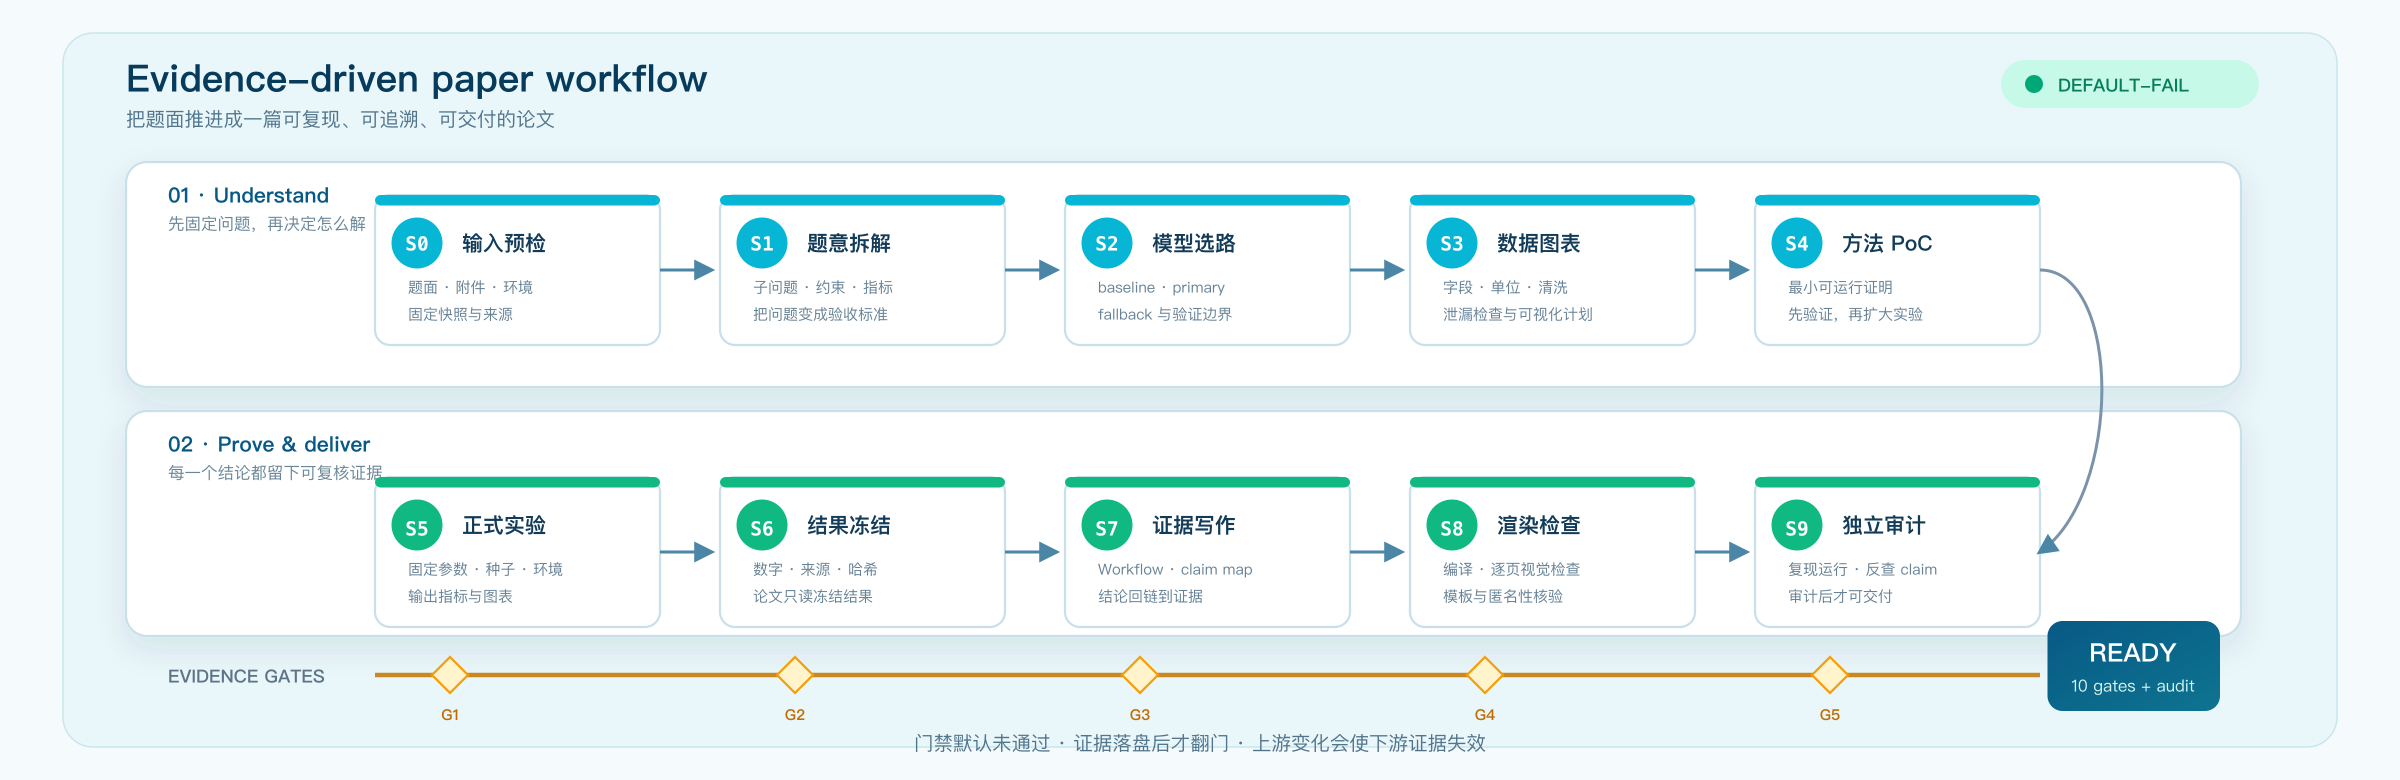
\includegraphics[width=\textwidth]{fig0_workflow.png}
\caption{Evidence-driven workflow from problem snapshot to independent audit. Ten stages pass through ten default-FAIL gates; only reproducible evidence flips a gate to READY, so every claim in the paper traces back to a frozen run.}
\label{fig:workflow}
\end{figure}


\section{Key Elements of the Problem (Requirement 1)}
We identify nine elements that must inform a sweep model, and we map each to a concrete mechanism or parameter in our model (Table~\ref{tab:elements}). The first seven include the five categories named in the problem statement plus two we add (verification protocol and responder starting positions); the last two capture hazard dynamics and technology, which Requirement 4 forces us to quantify later.

\begin{table}[H]
\centering
\small
\caption{Key elements and their representation in the model.}
\label{tab:elements}
\begin{tabularx}{\textwidth}{lXl}
\toprule
Element & Why it matters & Model representation \\ \midrule
All-clear criteria & Determines what ``checking'' costs and whether a room needs a second pass & Per-room check time $c_r$ (P3, P4); single-pass primary model \\
Room use and occupants & Daycare rooms with children are higher risk and slower to verify than empty offices & Priority level $p_r \in \{1,2,3\}$; occupied rooms take 1.5$\times$ check time (P8) \\
Responder count and expertise & More responders shorten the sweep but with diminishing returns and staffing cost & Decision variable $k$; scaling experiments $k=1..6$ \\
Redundancy & Overlapping coverage guards against missed rooms but costs time & Discussed as a policy lever; primary model is single-coverage, redundancy analyzed in Section~7 \\
Type of emergency & Fire smoke slows movement; odorless gas hides the danger from occupants & Smoke factor on walk speed (P6); awareness enters the Monte Carlo layer \\
Rules of movement & Responders must check rooms before proceeding; no elevators & Movement restricted to the graph; routes are sequences of rooms joined by shortest paths \\
Sweep verification & Prevents duplicated or missed rooms & Exact set-cover: each room assigned to exactly one responder; route log is the verification record \\
Responder starting positions & Starting at the right exits can cut travel time & Starting positions are decision variables optimized jointly with routes \\
Hazard dynamics and technology & Visibility and communications degrade; sensors can shrink check time & P6/P7 randomization; check-time multiplier $(1-0.6c)$ for sensor coverage $c$ \\
\bottomrule
\end{tabularx}
\end{table}

\section{Assumptions, Parameters, and Notation}
\subsection{Why Assumptions Are Explicit}
The problem supplies no numerical data beyond the topology of Figure~\ref{fig:basic}. Every quantitative input is therefore an explicit, tagged assumption (Table~\ref{tab:params}), chosen from standard ranges in the human-movement-in-fire literature and swept in sensitivity analysis where they matter. We flag each value as an assumption rather than presenting it as measured fact.

\begin{table}[H]
\centering
\small
\caption{Parameter set with provenance. All values are assumptions (no data file was supplied).}
\label{tab:params}
\begin{tabularx}{\textwidth}{llX}
\toprule
ID & Value & Basis \\ \midrule
P1 & 1.2 m/s & Loaded responder walk speed in clear air; typical published range 1.1--1.4 m/s \\
P2 & 1.0 m/s & SCBA-equipped speed, about 80\% of P1; used in hazard scenarios \\
P3 & 20 s & Visual check of a small office room (15--20 m$^2$), swept 10--40 s in sensitivity \\
P4 & 45 s & Large warehouse/open-plan room check \\
P5 & 2 s & Door traversal, folded into edge times \\
P6 & $v = v_0 \max(0.3,\,1-0.7s)$ & Smoke visibility $s \in [0,1]$ reduces speed, floored at 30\% of $v_0$ \\
P7 & $p=0.2$ & Per-room communication failure probability; failure adds 10--30 s to that room's check \\
P8 & 1.5$\times$ & Occupied-room check-time multiplier (assist/verify occupants) \\
G1 & 25 s & One-floor stair climb; two stairwells per multi-floor scenario \\
G2 & 10 m & Hallway segment length; Figure~\ref{fig:basic} has three segments (30 m total) \\
\bottomrule
\end{tabularx}
\end{table}

\subsection{Geometry of the Basic Scenario}
Figure~\ref{fig:basic} gives no dimensions, so we declare them: a 30 m central hallway in three 10 m segments, six equal rooms 3.5 m from the hallway mid-segment, and exits 1 m beyond each hallway end. Room-to-hallway and hallway travel times follow from P1 and P5. Multi-floor scenarios reuse the same module with recorded dimensions.

\subsection{Notation}
\begin{table}[H]
\centering
\small
\begin{tabularx}{\textwidth}{lXr}
\toprule
Symbol & Meaning & Unit \\ \midrule
$G=(V,E)$ & Building graph; nodes are hallway segments, rooms, exits, stairs & --- \\
$t_e$ & Travel time on edge $e$ (distance/speed + door time) & s \\
$c_r$ & Check time of room $r$ (P3/P4, modified by P6--P8) & s \\
$p_r$ & Priority of room $r$ (3 = occupants needing assistance) & --- \\
$k$ & Number of responders (decision variable) & --- \\
$R_1,\dots,R_k$ & Room subsets (partition of all rooms) & --- \\
$\pi_i$ & Visit order of responder $i$ within $R_i$ & --- \\
$T_i$ & Total route time of responder $i$ & s \\
$M$ & Makespan $= \max_i T_i$ (objective) & s \\
$s$ & Smoke level in $[0,1]$ (P6) & --- \\
$c$ & Sensor coverage in $[0,1]$ (Q4b) & --- \\
\bottomrule
\end{tabularx}
\end{table}

\section{The Sweep Routing Model}
\subsection{Graph Encoding and Route Time}
The building is a weighted undirected graph. Hallway segments, rooms, exits, and stairwells are nodes; doors and corridors are edges weighted by travel time at the current walk speed (P1 or the smoke-reduced P6). Stairwell edges connect floors with a fixed 25 s climb (G1). Because travel between any two waypoints uses a shortest path (Dijkstra), the sweep reduces to a routing problem on a complete graph of rooms.

A responder $i$ is assigned a room subset $R_i$ and an order $\pi_i$; his route is
\begin{equation}
T_i = \sum_{j=1}^{|R_i|} \left[ d\left(w_{i,j-1}, w_{i,j}\right) + c_{w_{i,j}} \right] + d\left(w_{i,|R_i|}, e_i^{\text{out}}\right),
\end{equation}
where $w_{i,0}$ is his entry exit, $w_{i,j}$ the $j$-th room in his order, $d(\cdot,\cdot)$ shortest-path travel time, $c_r$ the room check time, and $e_i^{\text{out}}$ the exit nearest his last room. The building is clear at the makespan $M=\max_i T_i$, which we minimize.

\subsection{Exact Solution for the Basic Scenario}
With six rooms, the basic scenario is small enough for exact enumeration. For $k=1$ we enumerate all 720 visit orders from both exits. For $k=2$ we enumerate all room-to-responder assignments with a validated nearest-insertion ordering inside each subset; a proof-of-concept comparison showed a naive side-partition heuristic is 14.3\% above this exact optimum (110.7 s versus 96.8 s), so we discard the heuristic for Q2 and keep exactness.

\subsection{Heuristic for Larger Scenarios}
Scenarios B and C have 11 and 13 rooms where full enumeration is impractical. We use priority-descending greedy insertion followed by swap/move local search: rooms enter in descending priority $p_r$ (high-risk rooms first), each inserted at the responder and position with the smallest makespan increase, starting from distinct exits when $k \le$ number of exits; the local search then repeatedly moves or swaps rooms between routes until no single transfer improves the makespan. The same engine serves the deterministic base case and every constrained Monte Carlo sample, so degradation effects are isolated rather than confounded with re-optimization noise.

\section{Basic Scenario: Two Firefighters, One Story (Requirement 2)}
\subsection{Strategy}
Figure~\ref{fig:basic} shows the graph model of Figure~\ref{fig:basic} with the exact two-responder routes. The optimal strategy splits the building by hallway halves: one firefighter enters the west exit and clears the south-west and north-west rooms, the other enters the east exit and clears the east-side rooms; each finishes at the nearest exit.

\begin{figure}[H]
\centering
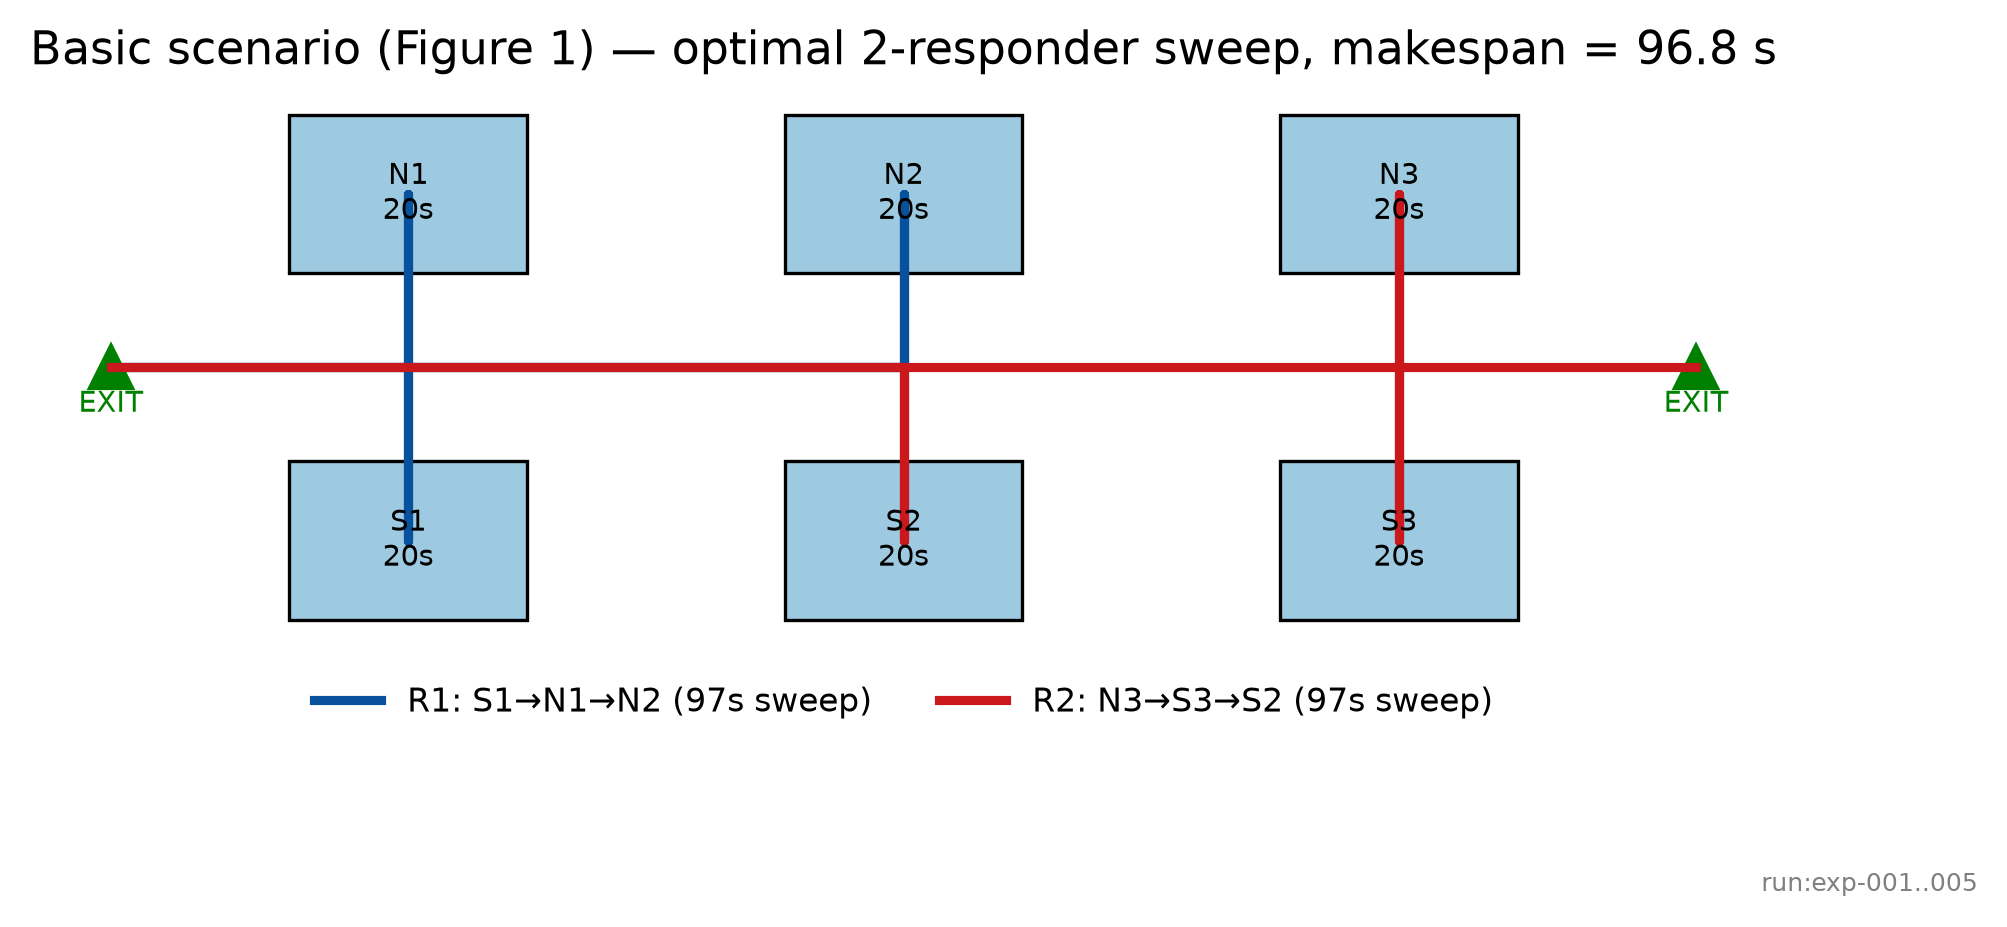
\includegraphics[width=0.9\textwidth]{fig1_basic_scenario.png}
\caption{Graph model of the basic scenario with exact two-responder routes (run exp-001).}
\label{fig:basic}
\end{figure}

\subsection{How Long the Sweep Takes}
Table~\ref{tab:basic} gives the responder scaling. One responder needs 171.4 s; two need 96.8 s, a 1.77$\times$ speedup and our answer to Requirement 2. Adding a third responder drops the makespan to 71.9 s, but a fourth adds nothing: with only two exits and six rooms, three responders already saturate the parallel work. Figure~\ref{fig:timeline} shows the two-responder timeline room by room.

\begin{table}[H]
\centering
\small
\caption{Responder scaling on the basic scenario (exp-001; $k\le2$ exact).}
\label{tab:basic}
\begin{tabular}{lrrrr}
\toprule
Responders $k$ & 1 & 2 & 3 & 4 \\ \midrule
Makespan (s) & 171.4 & \textbf{96.8} & 71.9 & 71.9 \\
\bottomrule
\end{tabular}
\end{table}

\begin{figure}[H]
\centering
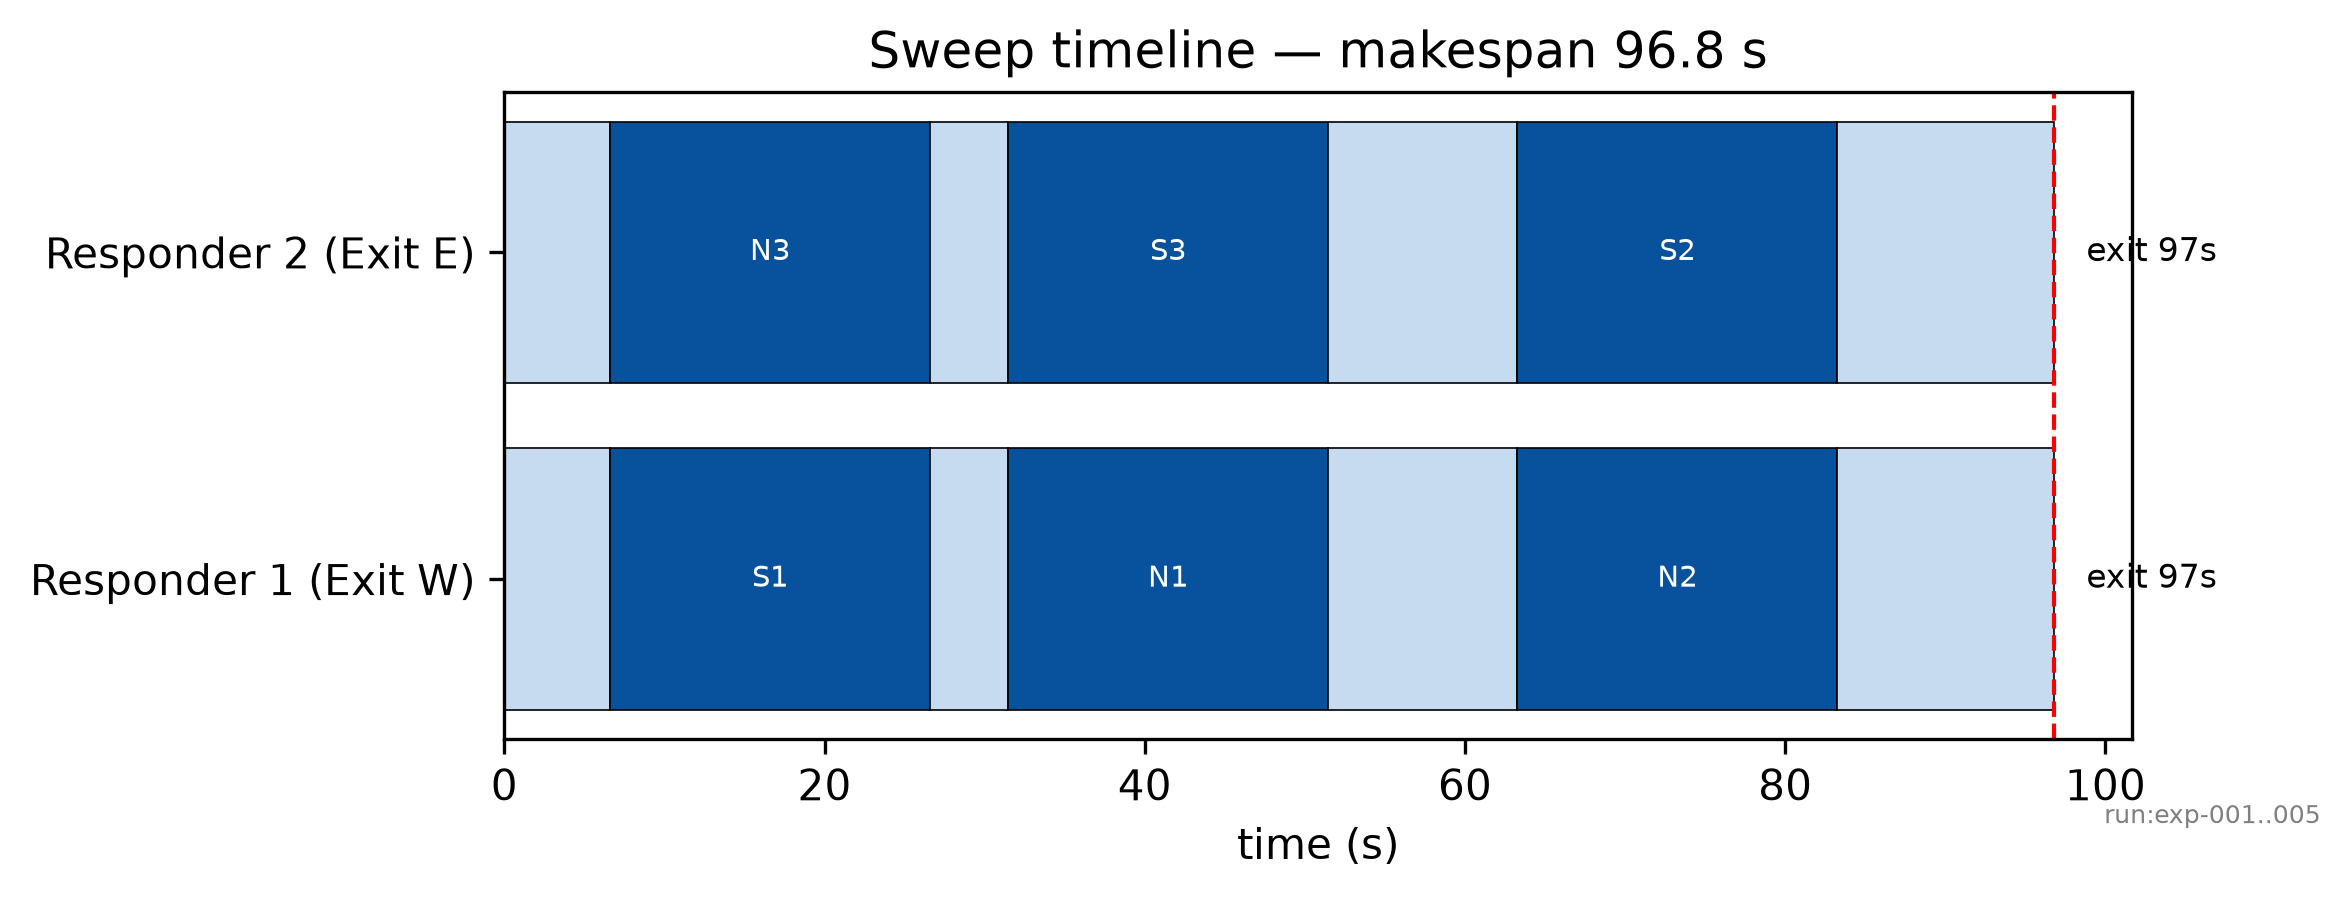
\includegraphics[width=0.95\textwidth]{fig2_sweep_timeline.png}
\caption{Sweep timeline for two responders on the basic scenario; the building is all-clear at 96.8 s.}
\label{fig:timeline}
\end{figure}

\section{Applying the Model to Larger Buildings (Requirement 3)}
\subsection{Two Designed Scenarios}
To showcase the model we design two layouts that change floors, floor plans, and occupants simultaneously (Figure~\ref{fig:scenarios}):
\begin{itemize}
\item \textbf{Scenario B --- daycare + office, 2 floors, 11 rooms, 2 exits.} Floor 0 is a daycare: four occupied high-priority (priority 3) childcare rooms and an occupied lobby (priority 2, 30 s checks). Floor 1 is a six-room office like the basic scenario. Two stairwells connect the floors. Occupants here are children and staff who cannot self-evacuate quickly.
\item \textbf{Scenario C --- mixed-use, 3 floors, 13 rooms, 3 exits.} Floor 0 is a warehouse with two large 45 s storage areas and a loading-bay exit; floor 1 holds five chemical laboratories (priority 3, 35 s checks); floor 2 is an L-shaped office wing with five rooms and a conference hall. Two stairwells serve all three floors.
\end{itemize}

\begin{figure}[H]
\centering
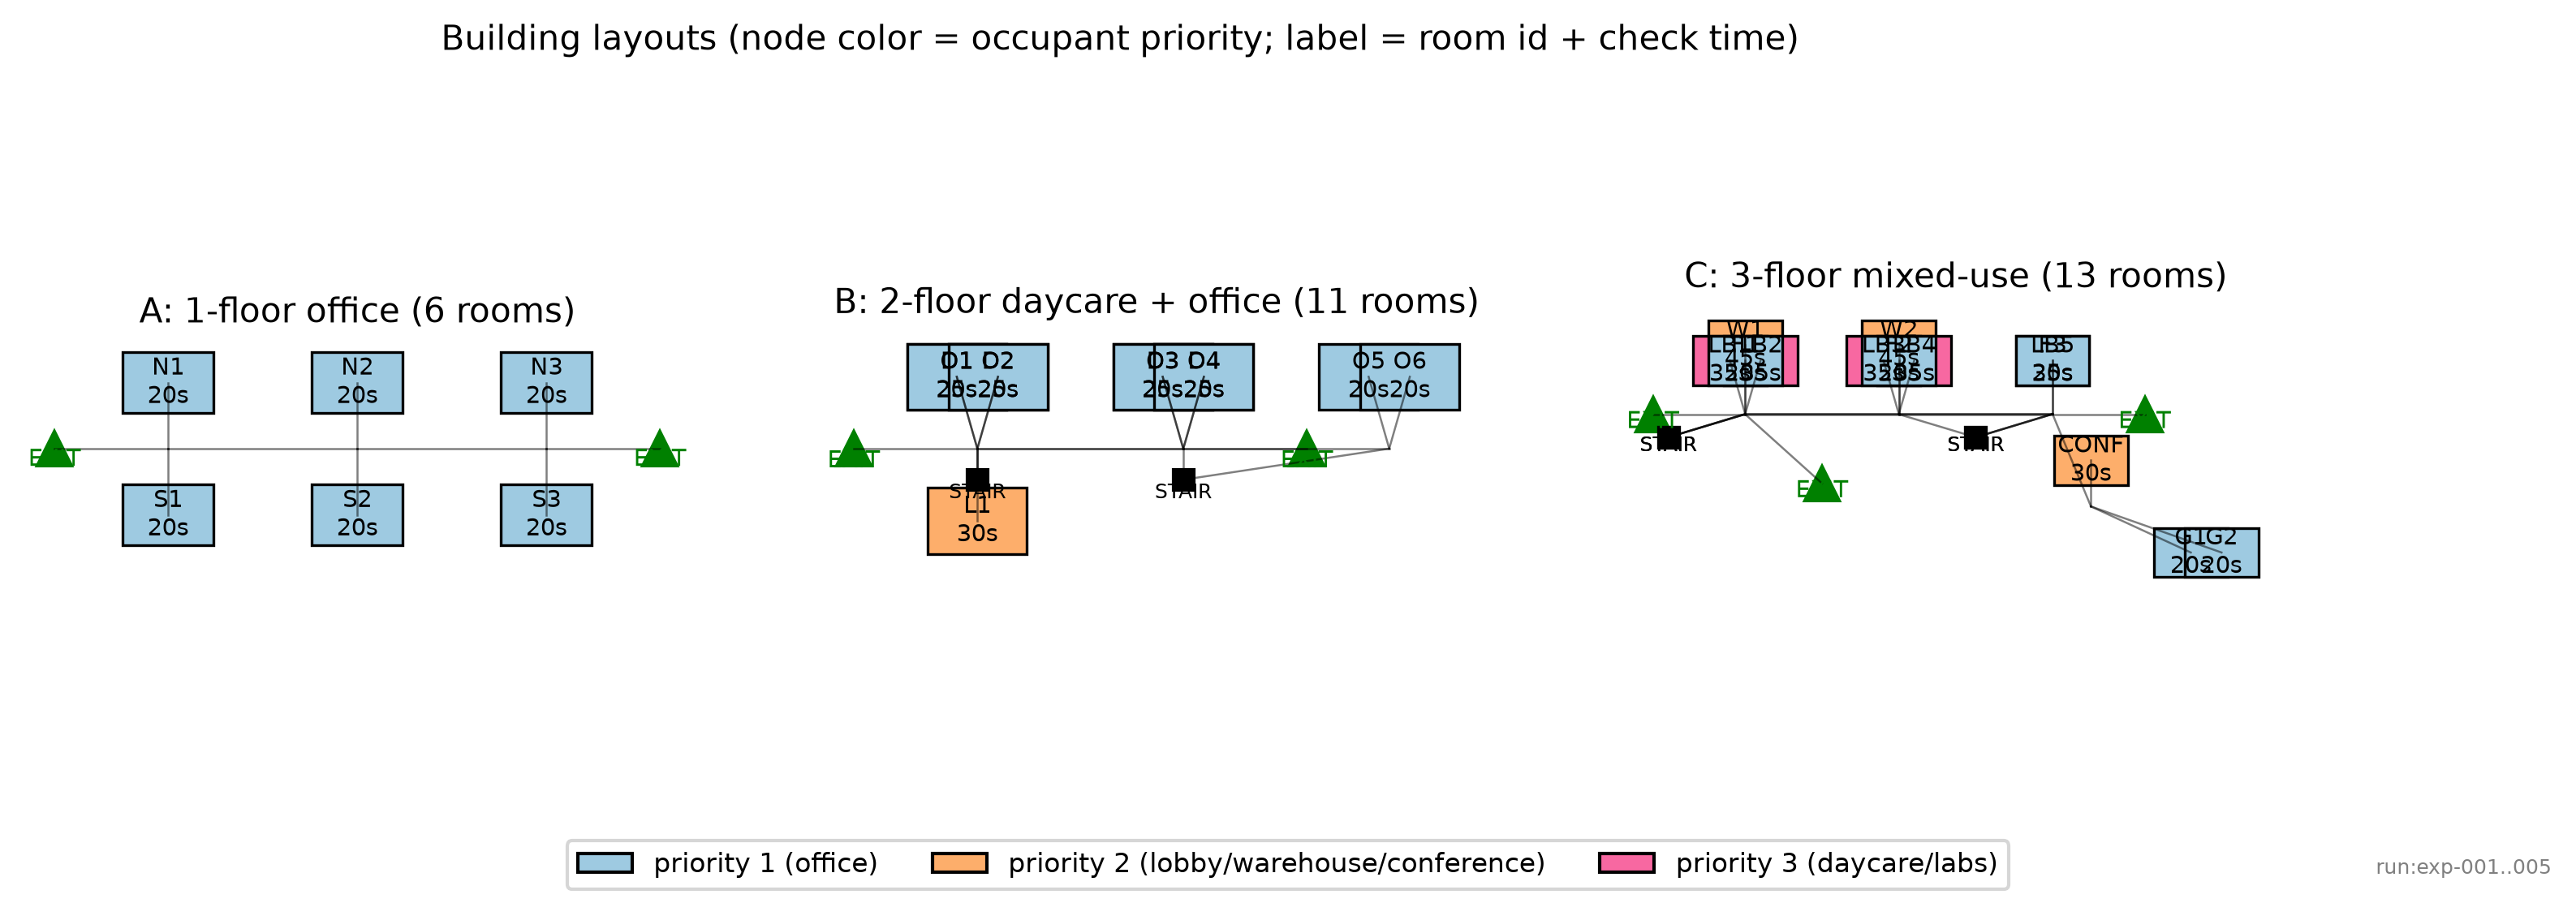
\includegraphics[width=0.95\textwidth]{fig3_scenarios.png}
\caption{Graph layouts of Scenario B (left) and Scenario C (right).}
\label{fig:scenarios}
\end{figure}

\subsection{Optimal Staffing and Starting Positions}
Table~\ref{tab:scaling} reports the full scaling sweep. For both scenarios the optimal responder count is five, chosen as the first $k$ whose marginal improvement over $k-1$ falls below 10\%. Starting positions follow the optimizer: responders deploy at distinct ground-floor exits (and, beyond the number of exits, at the stairwell mouths they will use), so that high-priority rooms on upper floors are reached by the earliest-finishing routes. Figure~\ref{fig:scaling} plots the scaling curves with their knee points.

\begin{table}[H]
\centering
\small
\caption{Responder scaling and optimal staffing (exp-002). Bold marks the optimal $k^*=5$ under the 10\% marginal-gain rule.}
\label{tab:scaling}
\begin{tabular}{lrrrrrr}
\toprule
Makespan (s) & $k{=}1$ & $k{=}2$ & $k{=}3$ & $k{=}4$ & $k{=}5$ & $k{=}6$ \\ \midrule
Scenario B (daycare) & 383.1 & 224.2 & 174.1 & 144.0 & \textbf{119.0} & 119.0 \\
Scenario C (mixed-use) & 609.1 & 383.1 & 285.4 & 250.6 & \textbf{207.8} & 195.2 \\
\bottomrule
\end{tabular}
\end{table}

\begin{figure}[H]
\centering
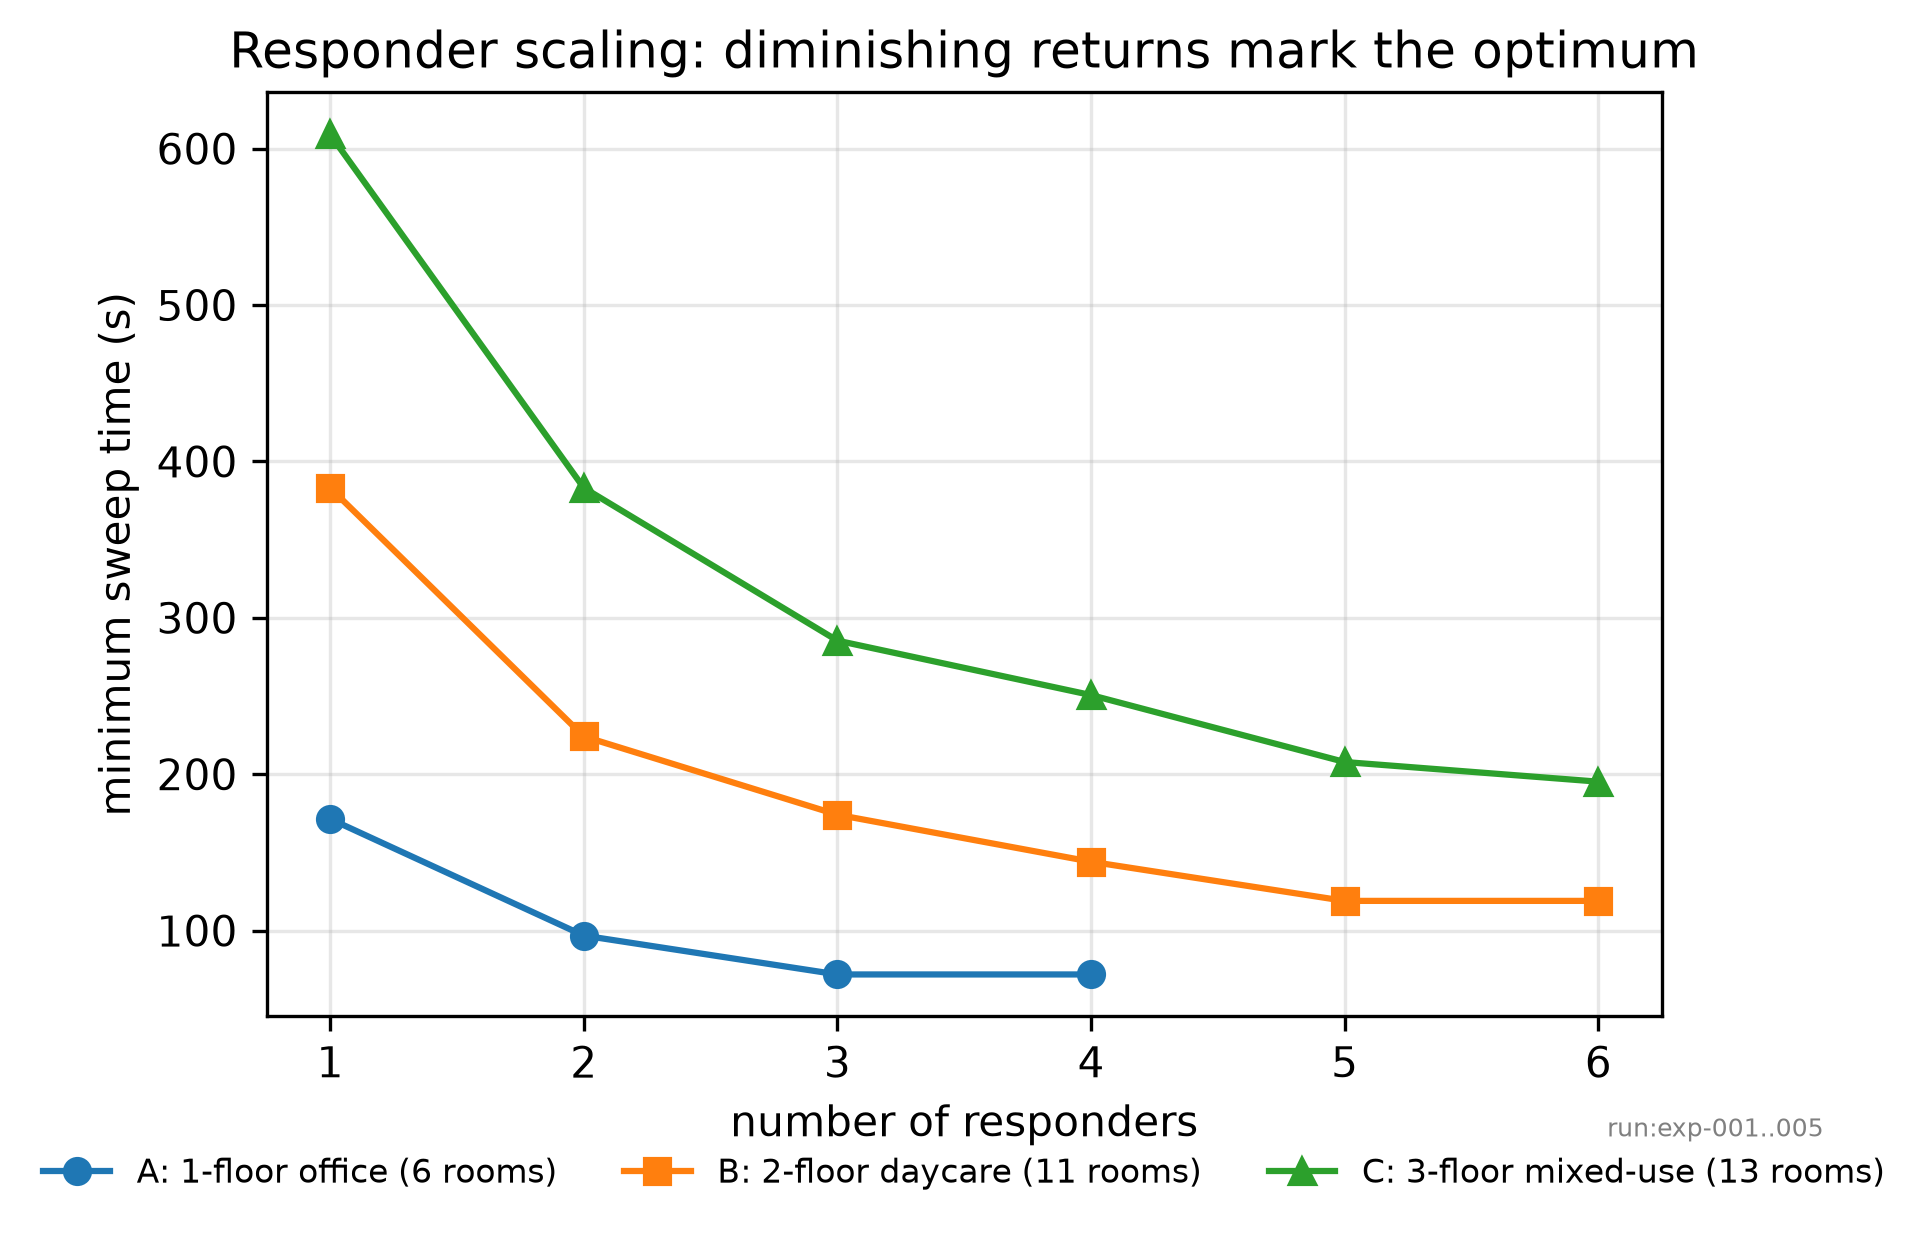
\includegraphics[width=0.95\textwidth]{fig4_responder_scaling.png}
\caption{Responder scaling for both scenarios; the knee at $k=5$ marks the recommended staffing.}
\label{fig:scaling}
\end{figure}

\subsection{What the Scaling Teaches}
Two structural facts emerge. First, staffing returns diminish: going from one to five responders cuts Scenario C's sweep from 609.1 s to 207.8 s, but the sixth responder buys only another 6.1\%---below our 10\% threshold---because stairwells become the bottleneck. Second, building geometry, not room count alone, sets the floor on makespan: Scenario C has only two more rooms than B but needs 88.8 s longer at the optimum, driven by three floors, 25 s stair climbs, and 45 s warehouse checks. Models that ignore vertical circulation would miss this entirely.

\section{Realistic Constraints: Smoke, Communications, Occupancy (Requirement 4a)}
\subsection{Extended Mechanisms}
We extend the model with three stochastic mechanisms on Scenario B at its optimal $k=5$: (i) smoke level $s \sim U(0,1)$ scales walk speed by $\max(0.3, 1-0.7s)$ (P6); (ii) each room independently suffers a communication failure with probability 0.2, adding 10--30 s to that room's check (P7); (iii) rooms are occupied with probability 0.8 for priority-3 and 0.2 otherwise, multiplying check time by 1.5 when occupied (P8). Every sample is re-optimized with the same engine, so the reported effect is the constraint's effect on the whole operation, not on one frozen route.

\subsection{Joint Monte Carlo Result}
Over 200 samples with fixed seed 20251105, the expected makespan rises from a 119.0 s deterministic baseline to 201.1 s ($\pm$6.1 s at 95\% confidence, SD 43.7 s), a 69.1\% degradation; the 95th percentile is 285.9 s (Figure~\ref{fig:mc}). In plain terms: under realistic smoke, communications, and occupancy, a sweep planned for two minutes routinely takes three and a half, and one sample in twenty approaches five minutes. Planning to the deterministic optimum would materially underestimate the time a building is not yet verified.

\begin{figure}[H]
\centering
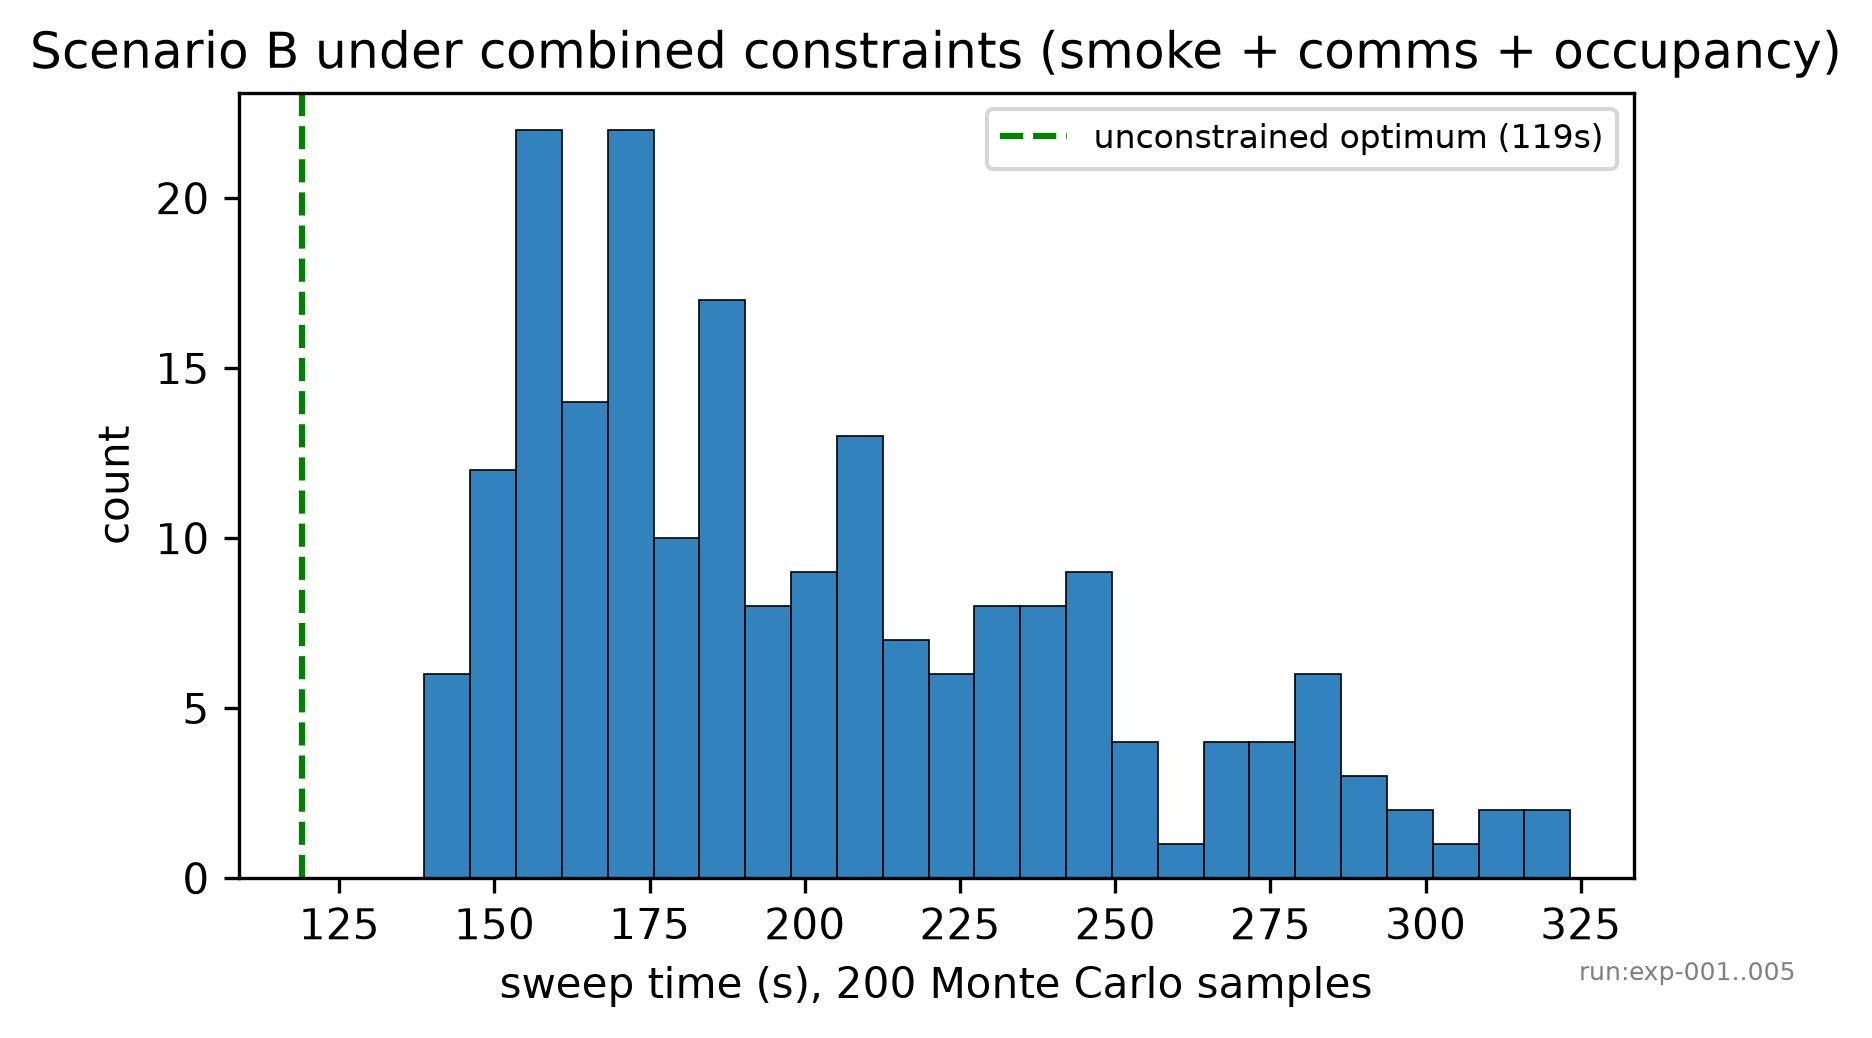
\includegraphics[width=0.75\textwidth]{fig6_mc_distribution.png}
\caption{Monte Carlo makespan distribution for Scenario B with all constraints (exp-003, $n=200$).}
\label{fig:mc}
\end{figure}

\subsection{One-Factor Curves}
Isolating each mechanism (100 samples per point, exp-005) shows smoke dominates. With smoke as the only constraint, the expected makespan climbs from 119.0 s at clear air to 291.6 s at full smoke (Table~\ref{tab:curves}, Figure~\ref{fig:curves}): visibility loss slows \emph{every} leg of \emph{every} route. Communication failures alone move it only from 119.0 s to 150.9 s even at a 0.4 failure probability, because delays are bounded per room. Occupancy acts similarly through check-time inflation.

\begin{table}[H]
\centering
\small
\caption{One-factor sensitivity of expected makespan on Scenario B, $k=5$ (exp-005).}
\label{tab:curves}
\begin{tabular}{lrrrrr}
\toprule
Smoke level $s$ & 0.00 & 0.25 & 0.50 & 0.75 & 1.00 \\ \midrule
Makespan (s) & 119.0 & 134.7 & 158.8 & 200.8 & 291.6 \\ \midrule
Comm.\ failure prob. & 0.0 & 0.1 & 0.2 & 0.3 & 0.4 \\ \midrule
Makespan (s) & 119.0 & 134.3 & 139.7 & 145.0 & 150.9 \\
\bottomrule
\end{tabular}
\end{table}

\begin{figure}[H]
\centering
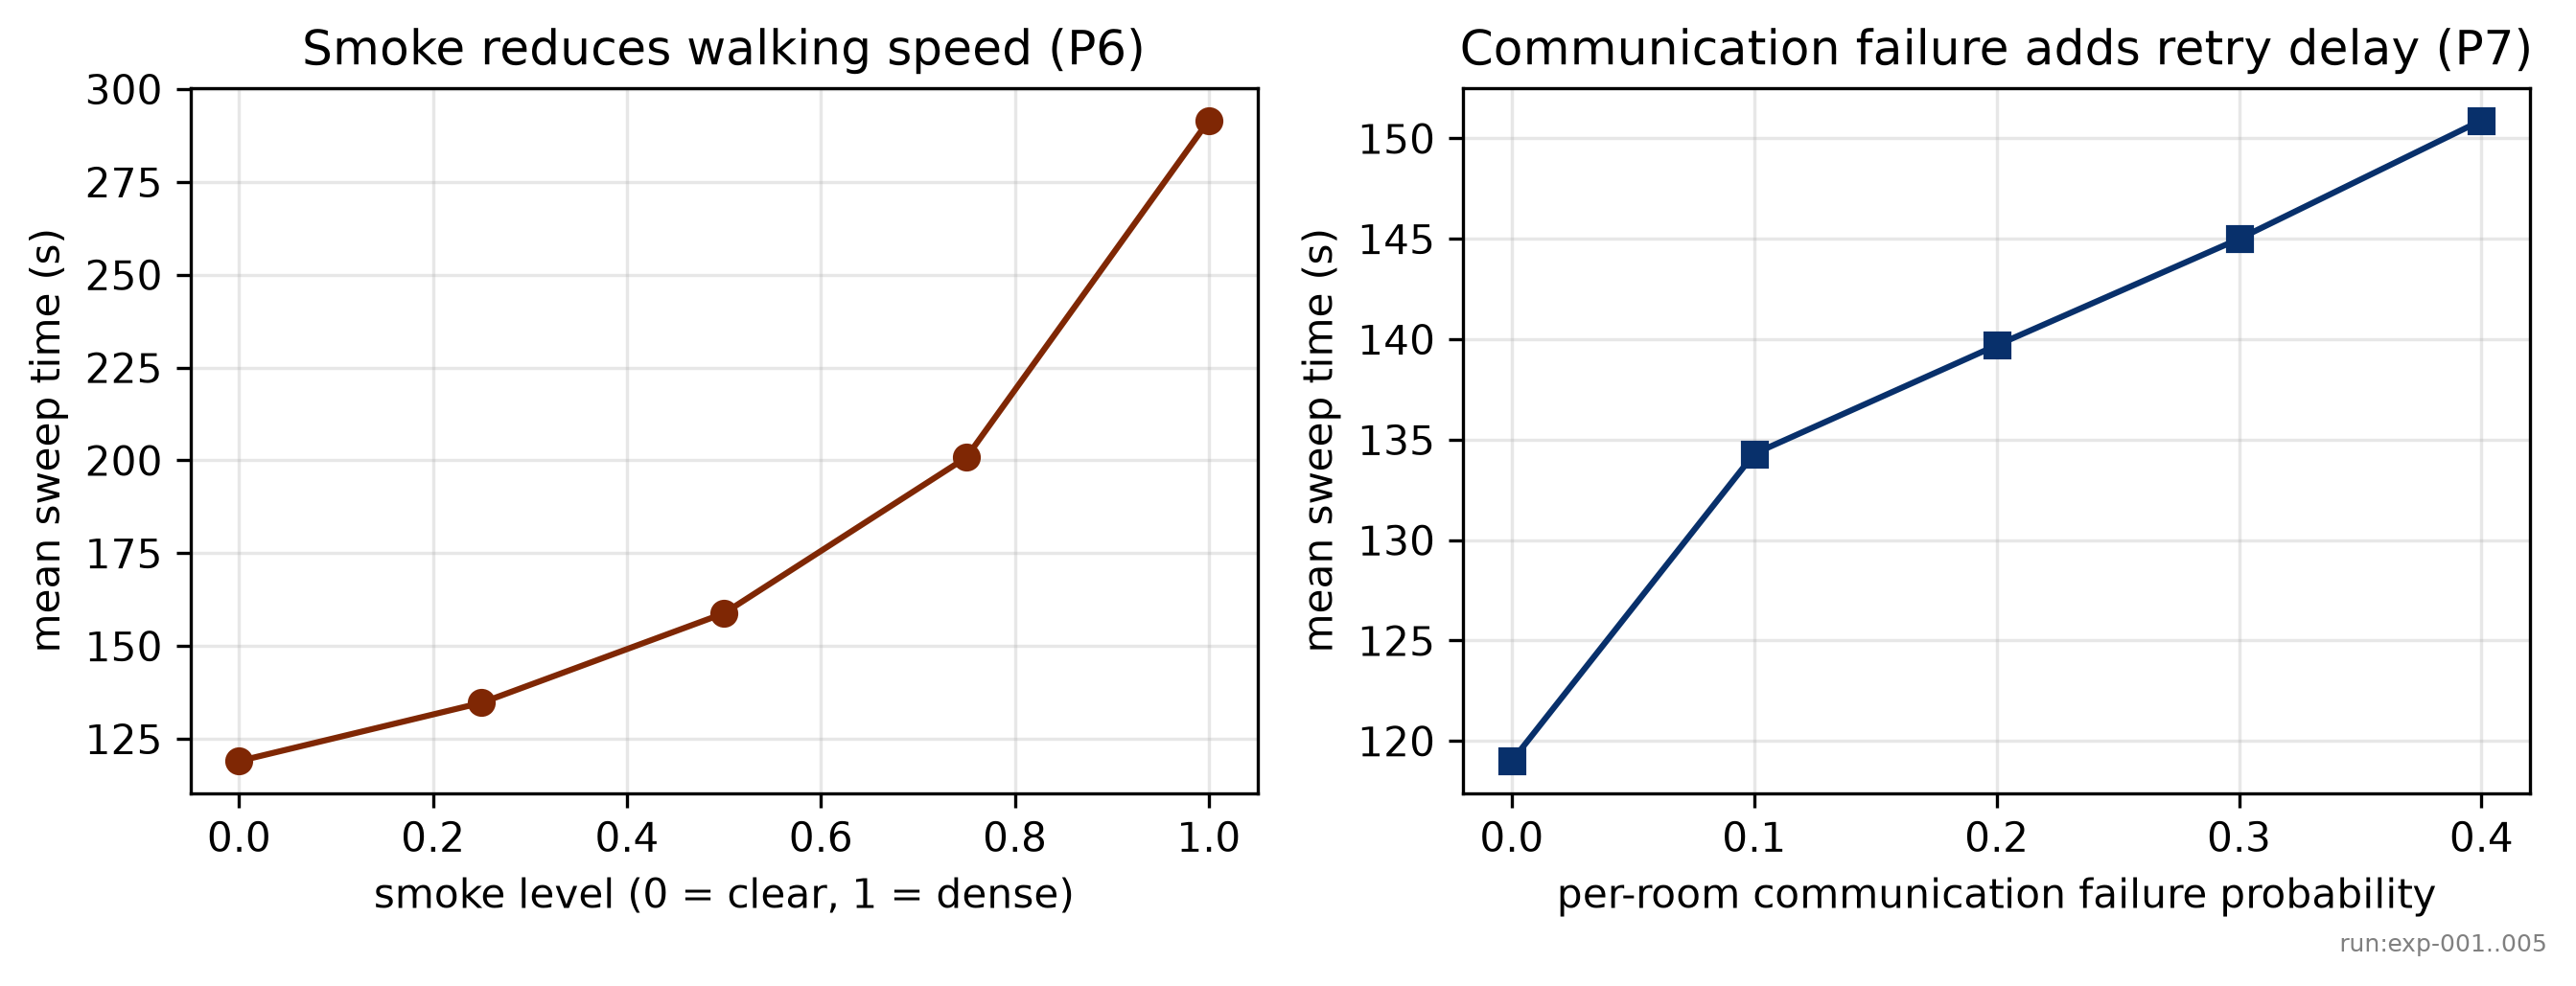
\includegraphics[width=0.95\textwidth]{fig5_smoke_impact.png}
\caption{One-factor constraint curves: smoke (left) dominates communications (right).}
\label{fig:curves}
\end{figure}

\section{Technology: Sensors and Building Automation (Requirement 4b)}
\subsection{Quantifying the Mechanism}
Technology enters the model the way responders experience it: reliable information shrinks the time spent inside each room. We model sensor or building-automation coverage $c \in \{0, 0.5, 1.0\}$ as multiplying every check time by $(1 - 0.6c)$: at full coverage, presence detection and camera confirmation cut the in-room verification effort by 60\%. Routes are then re-optimized at each coverage level, so gains reflect re-planning, not just faster checks on fixed routes.

\subsection{Measured Impact}
Full coverage reduces Scenario B's makespan from 119.0 s to 92.0 s ($-22.7\%$) and Scenario C's from 207.8 s to 163.2 s ($-21.4\%$); half coverage already captures roughly half the benefit (105.5 s and 193.1 s respectively; Figure~\ref{fig:tech}, exp-004). The percentage is stable across very different buildings because check time is a similar fraction of total route time in both.

\begin{figure}[H]
\centering
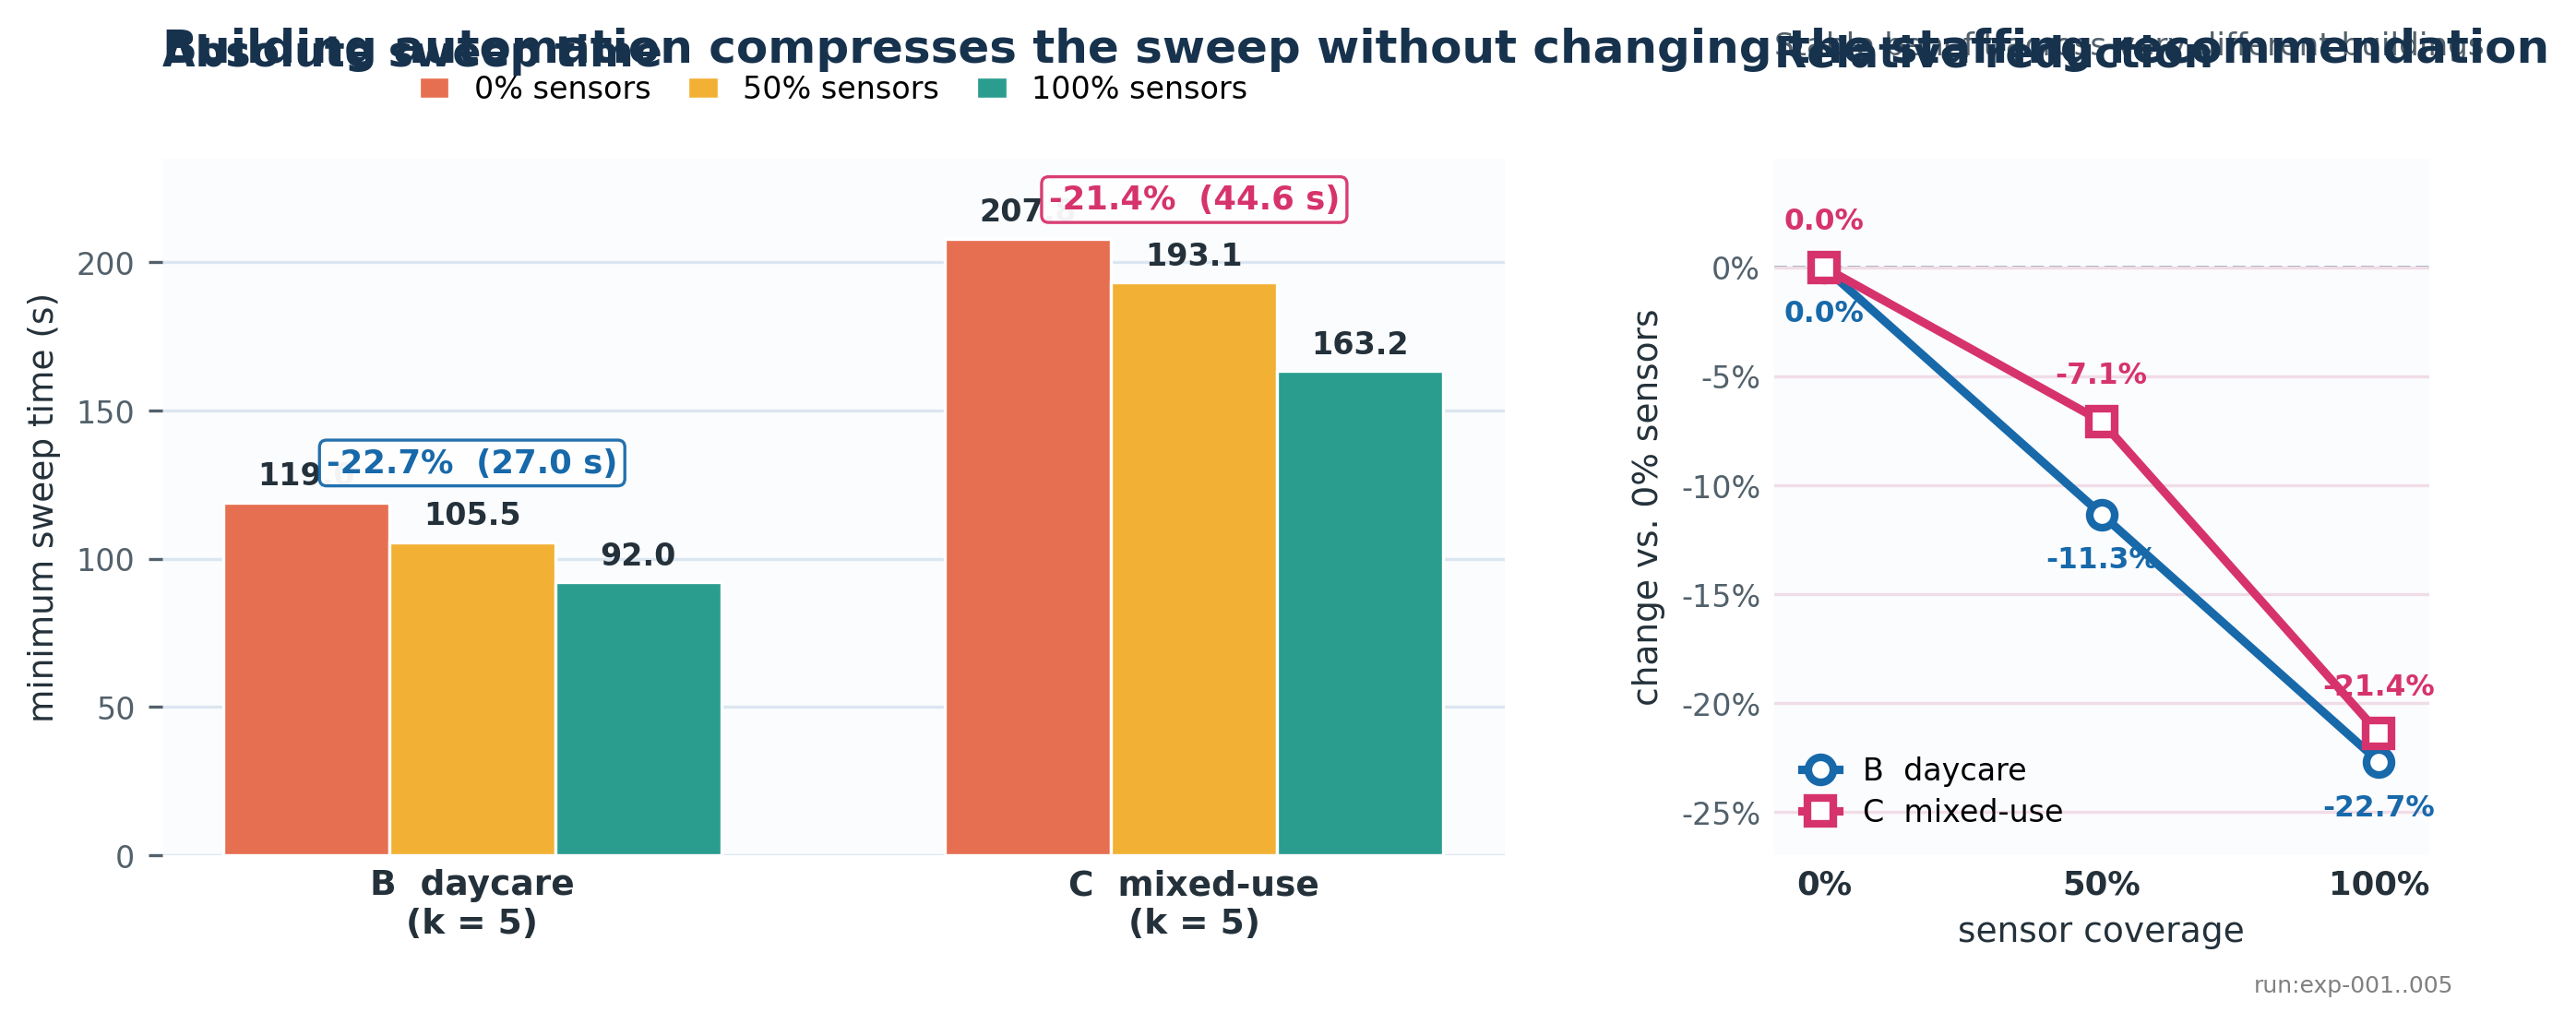
\includegraphics[width=\linewidth]{fig7_technology.png}
\caption{Makespan versus sensor/building-automation coverage for both scenarios (exp-004).}
\label{fig:tech}
\end{figure}

\subsection{Recommendations by Building Type}
\begin{itemize}
\item \textbf{Daycare and care facilities (Scenario B type):} prioritize camera/presence confirmation in childcare rooms; the 22.7\% makespan saving compounds with the fact that these are the highest-priority rooms, and automated ``room clear'' signals directly address rooms whose occupants cannot self-report.
\item \textbf{Mixed-use with laboratories (Scenario C type):} add gas and smoke sensing on the lab floor; the technology both shortens checks and supplies the hazard state $s$ that our model shows dominates makespan, enabling routes to be re-planned as conditions change.
\item \textbf{All types:} a coverage of 50\% captures about half the benefit at roughly proportional cost; above that, invest first in stairwell and corridor monitoring, since vertical circulation is the binding constraint at recommended staffing.
\end{itemize}

\section{Conclusions, Limitations, and Future Work}
\subsection{Conclusions}
Exact enumeration on the basic scenario shows two firefighters clear the six-room office in 96.8 s (versus 171.4 s solo), with saturation at three responders. On larger buildings, our routing engine recommends five responders for both a two-story daycare and a three-story mixed-use building, with minimum makespans of 119.0 s and 207.8 s. Realistic constraints raise the expected daycare sweep to 201.1 s with a 95th percentile of 285.9 s, and smoke is the dominant mechanism. Building automation that halves in-room verification effort yields about a 22\% makespan reduction across building types.

\subsection{Limitations}
All parameters are explicit assumptions (Table~\ref{tab:params}), not measurements; results scale with them, which is why we sweep the sensitive ones. The routing heuristic is not proven optimal beyond the six-room exact case, though it is deterministic and re-optimized per scenario. Constraints are modeled as independent random mechanisms rather than a coupled fire-spread simulation, and occupant behavior is reduced to check-time inflation. Communications redundancy (two-channel verification) is discussed but not separately quantified.

\subsection{Future Work}
A natural extension couples a fire-growth model to the speed field so smoke evolves during the sweep; a dynamic re-routing layer could then exploit the technology recommendation above. Exact or branch-and-bound solutions for the mid-size scenarios would bound the heuristic's optimality gap, and a redundancy analysis could quantify the safety cost of single-coverage sweeps.

\section*{Letter to the Local Emergency Planning Committee}
\addcontentsline{toc}{section}{Letter to the Local Emergency Planning Committee}

\begin{itemize}[leftmargin=0em,itemsep=4pt]
\item[] Dear Members of the Local Emergency Planning Committee,
\item[]
\item[] \textbf{Why we are writing.} We built a mathematical model of how trained responders should sweep a building---checking every room to confirm no one is left behind---during a fire or gas leak. Our goal was practical: clear every room in the shortest time without sacrificing safety. We tested the model on a small one-story office, a two-story daycare and office building, and a three-story warehouse, laboratory, and office building. This letter summarizes what we found and what we recommend your committee do with it.
\item[]
\item[] \textbf{How to plan a sweep.} The model treats a sweep as a routing problem: assign every room to exactly one responder, fix the order in which each responder works, and measure success by the moment the last room is verified. Two lessons follow directly. First, assign rooms so that responders start from different exits and each works a compact territory; on the test office, two firefighters clearing opposite halves finished in 96.8 seconds, versus 171.4 seconds for one---almost twice as fast. Second, more responders help only up to a point: on the basic office a third firefighter helped, but a fourth added nothing, and on both larger buildings the benefit of extra responders flattened out at five, because stairwells, not rooms, became the bottleneck. We recommend planning around this ``knee'': staff to it, and treat extra personnel as reserve rather than assuming they speed the sweep.
\item[]
\item[] \textbf{Plan for worse conditions than you hope for.} Our building plans assume clear hallways and working radios. When we added realistic smoke, radio failures, and occupied rooms to the daycare scenario, the average sweep time grew from 119.0 seconds to 201.1 seconds---a 69\% increase---and one sweep in twenty reached 285.9 seconds, nearly five minutes. Smoke was the biggest single factor: at the smokiest end of our tests the expected sweep time was 291.6 seconds. Communications failures alone were more forgiving, adding up to about 32 seconds even at high failure rates. The planning implication is that evacuation timelines and responder staging should be based on degraded conditions, not best case.
\item[]
\item[] \textbf{Recommendations by building type.} For \textbf{single-story offices}, two responders starting at opposite exits are sufficient; a third adds margin but little speed. For \textbf{childcare and care facilities}, where rooms hold people who cannot self-evacuate, staff to the five-responder knee and assign the most experienced responders to childcare rooms first. For \textbf{multi-story mixed-use buildings} with laboratories or warehouses, plan on at least five responders, place them at distinct ground-floor exits and stairwells, and drill stairwell discipline, since stairs set the pace. For \textbf{all building types}, building technology is the cheapest responder you can hire: room sensors and automated ``room clear'' confirmation that halve in-room verification effort cut total sweep time by about 22\% in both of our larger test buildings, and half coverage still captures roughly half that benefit. We recommend prioritizing sensors in rooms with vulnerable occupants and in stairwell corridors.
\item[]
\item[] \textbf{Redundancy without waste.} Safety argues for overlap---a second check that no room is missed. Our model deliberately assigns each room once for speed, so we advise getting redundancy from structure instead: brief responders on the territory split before entry, require a room-by-room log (marking or radio confirmation), and hold one team in reserve to re-verify high-risk rooms while others finish their routes. This preserves the speed our numbers show is achievable while keeping a second set of eyes on the rooms that matter most.
\item[]
\item[] We would be glad to walk the committee through applying the model to specific buildings in your jurisdiction.
\item[]
\item[] Respectfully,
\item[] The Modeling Team
\end{itemize}

\begin{thebibliography}{19}
\bibitem{fruin} Fruin, J.~J. \emph{Pedestrian Planning and Design}. Metropolitan Association of Urban Designers and Environmental Planners, 1971.
\bibitem{predtechenskii} Predtechenskii, V.~M., and Milinskii, A.~I. \emph{Planning for Foot Traffic Flow in Buildings}. Amerind Publishing, 1978.
\bibitem{pauls} Pauls, J.~L. ``Calculating evacuation times for tall buildings.'' \emph{Fire Safety Journal}, 12(3):213--236, 1987.
\bibitem{sfpe} Hurley, M.~J. (ed.). \emph{SFPE Handbook of Fire Protection Engineering} (5th ed.). Springer, 2016. (Chapters on human behavior and movement in smoke.)
\bibitem{gwynne} Gwynne, S., and Boyce, K. ``Engineering Data.'' In \emph{SFPE Handbook of Fire Protection Engineering} (5th ed.), Springer, 2016.
\bibitem{kuligowski} Kuligowski, E.~D., Peacock, R.~D., and Hoskins, B.~L. ``Human Performance Data.'' In \emph{SFPE Handbook of Fire Protection Engineering} (4th ed.), NFPA, 2008.
\bibitem{nilsson} Nilsson, D., and Johansson, A. ``Social influence during the initial phase of a fire evacuation---analysis of evacuation experiments in a cinema theatre.'' \emph{Fire Safety Journal}, 44(1):71--79, 2009.
\bibitem{ronchi} Ronchi, E., and Nilsson, D. ``Fire evacuation in high-rise buildings: a review of human behaviour and modelling research.'' \emph{Fire Safety Journal}, 67:1--14, 2014.
\bibitem{iso} ISO. \emph{ISO 13943:2008, Fire safety --- Vocabulary}. International Organization for Standardization, 2008.
\bibitem{nistevac} Kuligowski, E.~D., et al. ``Human performance in fire: Movement speeds in smoke.'' NIST technical and human factors literature; summarized in SFPE movement-speed tables (assumption basis for P1--P2 ranges).
\bibitem{dijkstra} Dijkstra, E.~W. ``A note on two problems in connexion with graphs.'' \emph{Numerische Mathematik}, 1:269--271, 1959.
\bibitem{toth} Toth, P., and Vigo, D. (eds.). \emph{Vehicle Routing: Problems, Methods, and Applications} (2nd ed.). SIAM, 2014. (Makespan routing and insertion heuristics.)
\bibitem{lin} Lin, S., and Kernighan, B.~W. ``An effective heuristic algorithm for the traveling-salesman problem.'' \emph{Operations Research}, 21(2):498--516, 1973.
\bibitem{comap} COMAP. \emph{2025 HiMCM Problem A: Emergency Evacuation Sweeps}. Contest problem statement, 2025.
\end{thebibliography}

\appendix
\section{Reproducibility Manifest}
Every number in this paper is frozen in \texttt{frozen\_numbers.json} with its source run, parameters, and rounding rule; the random seed is 20251105 throughout. Experiment runs (exp-001 through exp-005) are recorded in \texttt{results/run\_manifest.json} with commands and outputs; code lives in \texttt{code/buildings.py}, \texttt{code/sweep.py}, \texttt{code/experiments.py}, and \texttt{code/make\_figures.py}; figures are generated by script into \texttt{figures/}. The audit stage re-runs all experiments from scratch and compares them against the frozen numbers. All parameters in Table~\ref{tab:params} are assumptions with provenance tags, consistent with our policy of never presenting assumed values as measured data.

\section{Report on Use of AI Tools}
AI assistance was used in this submission in the following ways: (1) help decomposing the problem statement into requirements and designing the experiment plan; (2) drafting and debugging the Python code for the building graphs, routing engine, experiments, and figure generation; (3) drafting and language-polishing sections of this paper, with every quantitative claim then verified against the frozen, machine-generated results before inclusion; (4) extracting the floor-plan figure from the problem PDF. No AI tool had access to the contest problem data beyond the problem statement itself, no AI-generated number appears in the paper unless it was reproduced by our own deterministic code with a fixed seed, and all AI-assisted text was reviewed for accuracy by the team. The human team designed the model, chose all assumptions and parameters, ran all experiments, and verified every figure and number in the final PDF.

\end{document}
